\chapter{SysML and ClassicalB}
\label{sec:sysML-B}

This section describes the approach of combining SysML modeling with
the B Method. The technical realization is shown in Figure
\ref{fig:classical-b-toolchain}. Modeling starts in SysML based on the
tool Papyrus. At the current stage of the project, it is undefined
which SysML elements and diagrams will be used. This must be well
defined to ensure that a transformation from SysML to Classical B is
semantically correct. To ensure this, the approach suggest the use of
the \emph{Object Constraint Language (OCL)} or the \emph{Eclipse
  Validation Framework} for validating the SysML model according to
defined modeling guidelines. Such guidelines may restrict the usage of
certain modeling elements and may enforce certain naming conventions.

The validated SysML model will be transformed to a Classical B model
with a model to text transformation language (e.g. Xtend2). That B
model is considered as read-only and is only allowed to be further
refined. From that point, the existing Atelier B toolchain will be
used for refining the model until reaching the implementation
model. Provers support the V\&V activities and the open source code
generator c4g is capable of generating C code.

The proposed toolchain is intended to be a first version. The yellow
boxes in Figure \ref{fig:classical-b-toolchain} indicate non existing
software artifacts that have to be developed within the openETCS
project. Furthermore, it is desirable to move parts from the Atelier B
tool into Eclipse. 

\begin{figure}
  \centering
  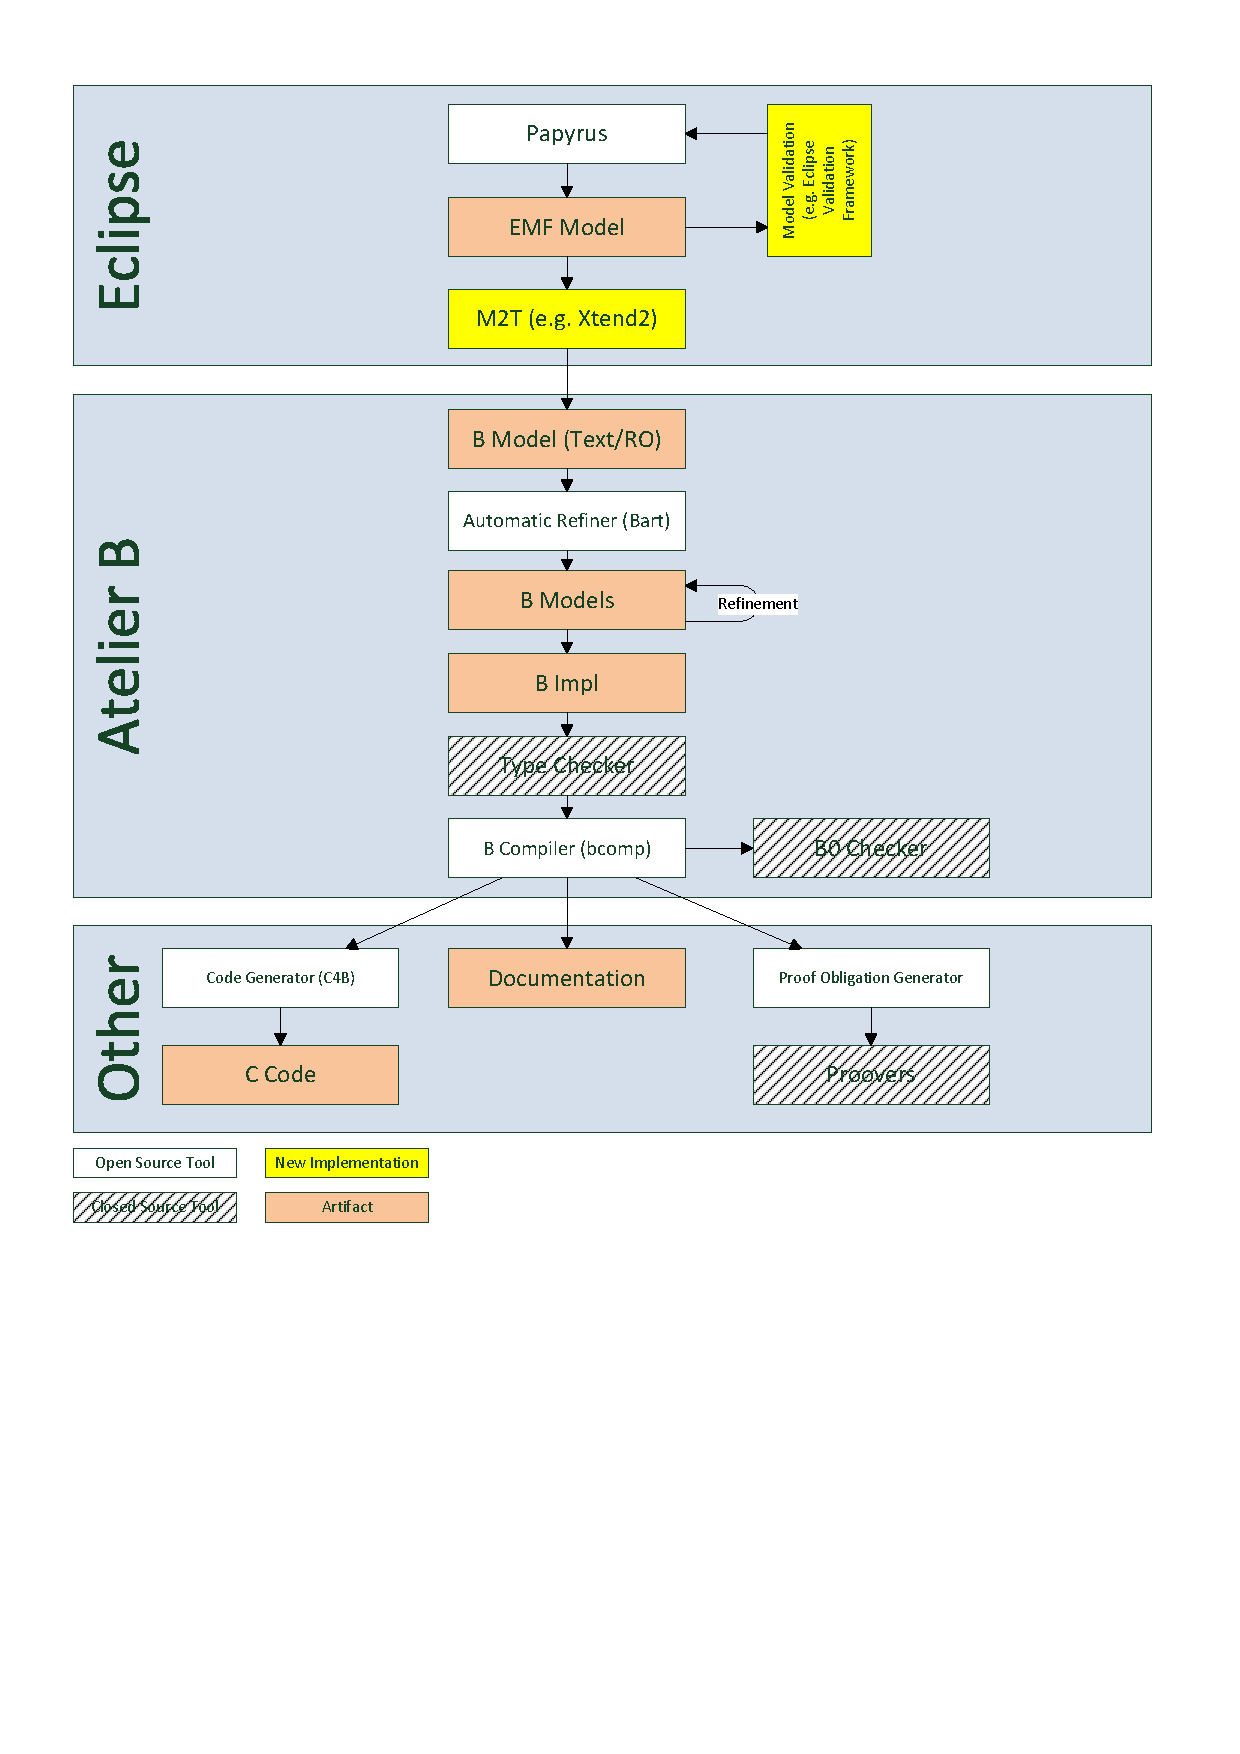
\includegraphics[width=6in]{images/classical_b_toolchain.pdf}
  \caption{Technical overview of the Papyrus and Classical-B toolchain}
  \label{fig:classical-b-toolchain}
\end{figure}


In Table \ref{tab:classical-b-tools} the list of tools used in the
proposed toolchain is given.

\begin{center}
\begin{table}
  \begin{tabular}{ l | l | l }
    Tool                               & License & Link \\ 
    \hline \hline
    Bart (B Automatic Refinement Tool) & GPL & \url{http://sf.net/projects/bartrefiner/} \\ \hline
    Atelier B GUI                      & GPL & \url{http://sf.net/projects/atelierbgui/} \\ \hline
    Bcomp (B Compiler)                 & GPL & \url{http://sf.net/projects/bcomp/} \\ \hline
    C4b (C Code Generator)             & GPL & \url{http://sf.net/projects/c4b/} \\ \hline
    \hline
  \end{tabular}
  \caption{Tools used in the Classical B toolchain}
  \label{tab:classical-b-tools}
\end{table}
\end{center}

\section{Description of the approach for OpenETCS design process}

Taking into account the results presented in Section
\ref{sec:results}, the proposed toolchain completely covers both, the
system phase as well as the software phase (see
Fig. \ref{fig:results}). On system analysis level, SysML with Papyrus
would be used for modeling the SSRS. Also for the sub-system semi
formal model, which will be created during the sub-system formal
design phase, it is proposed to use SysML with Papyrus. The finished
models will then be transformed to B models, to perform further
development steps according to the B method.

For both, the sub-system strictly formal model and the software
semi-formal model it is proposed to use the B method. The development
of the B models will be done by further refining the read-only B
model, generated from the SysML model. It has to be investigated where
\emph{exactly} the transition between SysML and the B model will be
done. In particular, it is currently unclear which SysML language
constructs and diagrams will be used and transformed to B. The
structure described in SysML with \emph{Block Definition Diagrams
  (BDD)} and \emph{Internal Block Diagram (IBD)} are obviously prime
candidates for a transformation to B, but which behavior diagram can
and will can be transformed is still under investigation.

The last part of the development process, the code generation, is
performed with an existing code generator tool.

\section{Integration of the approach with SysML/Papyrus}

\begin{todo_comment}
How the proposed approach can be integrated with the SysML/ Papyrus selected for the high level of design process ?
\end{todo_comment}

On the technical side, the integration will be performed by utilizing
the EMF framework of Eclipse. With an appropriate transformation
language (e.g. Xtend), the SysML model can be transformed to a textual
B model. If it is advantageous to perform the transformation with an
intermediate B meta-model and an a mode-to-model transformation (see
Fig. \ref{}) is under investigation.

The semantic integration of SysML and B method imposes a greater
challenge. There already exist literature regarding the alignment of
SysML and the B method. The work in \cite{} provides such an alignment
focusing on V\&V, which could be used as a base for further research
which consider in particular the openETCS requirements.


\section{Integration of the approach with Eclipse}

\begin{todo_comment}
How the proposed approach can be integrated with the Eclipse, selected as platform for OpenETCS tool chain ?
\end{todo_comment}

\section{Benefits versus OpenETCS requirements}

\begin{todo_comment}
Discuss the benefits in regards of OpenETCS requirements and expected results.
\end{todo_comment}

\section{Shortcommings versus OpenETCS requirements}

\begin{todo_comment}
Discuss the shortcommings in regards of OpenETCS requirements and expected results.
\end{todo_comment}

\section{On going work for openETCS project}

\begin{todo_comment}
Which are the elements to clarify, to specify or to develop, in order the approach suit the openETCS process ?

How can we evaluate and plan this work ?

which skills is needed ?
\end{todo_comment}

\section{Conclusion and other comments}
